\chapter{Canonical Correlation}
\label{cancor}

\section{Canonical variates}
\label{canvar}

\section{Interpretation}
\label{canint}
%%%%%\chapter{Canonical Correlation}

In canonical correlation, we are interested in the relationship between two sets of variables.   We do this by creating linear combinations $\boldsymbol{U} = \boldsymbol{a_{1} x_{1}} + \boldsymbol{a_{2} x_{2}} + \cdots + \boldsymbol{a_{p} x_{p}}$ and  $\boldsymbol{V} = \boldsymbol{b_{1} y_{1}} + \boldsymbol{b_{2} y_{2}} + \cdots + \boldsymbol{b_{q} y_{q}}$ such that the correlation between $\boldsymbol{U}$ and $\boldsymbol{V}$ is as high as possible.


To do this, we need to work out the correlation matrix, and partition it:


\begin{displaymath}
\begin{array}{ccccccc} & x_{1} & \ldots & \_{p} & y_{1} & \ldots & y_{q} \end{array}
\end{displaymath}
\begin{displaymath}
\begin{array}{c} x_{1} \\ \vdots \\ x_{p} \\y_{1} \\ \vdots \\y_{3}\end{array}
\left( \begin{array}{ccc|ccc} &&&&&\\&A_{p \times p}& &C_{p \times q}&\\&&&&&\\
\hline
&&&&&\\&C_{q \times p}& &B_{q \times q}&\\&&&&&\\ \end{array} \right)
\end{displaymath}

Having done this, we calculate the matrix:

\begin{displaymath}
\boldsymbol{B^{-1}C^{T}A^{-1}C}
\end{displaymath}

and find the associated eigenvalues (in descending order)  $\lambda_{1} > \lambda_{2} > \ldots > \lambda_{r}$.   The corresponding eigenvectors $\boldsymbol{b_{1}}, \boldsymbol{b_{2}}, \ldots, \boldsymbol{b_{r}}$ give the coefficients of the Y variables.

So: 

\begin{displaymath}
\boldsymbol{v_{i}} = \boldsymbol{b_{i}^{T}} \boldsymbol{Y}
\end{displaymath}

where $\boldsymbol{b_{i}} = \left(\begin{array}{c} b_{i1} \\ \vdots \\ b_{iq} \end{array} \right)$ and $\boldsymbol{Y} = \left(\begin{array}{c} \boldsymbol{y_{1}} \\ \vdots \\ \boldsymbol{y_{q}} \end{array} \right)$, or in longhand:

\begin{displaymath}
\boldsymbol{v_{i}} = b_{i1} \boldsymbol{y_{1}} + \cdots + b_{iq} \boldsymbol{y_{q}}
\end{displaymath}

Having calculated these, it is possible to solve the coefficients for the X variables:

$a_{1} = \boldsymbol{A^{-1} C b_{1}}, a_{2} = \boldsymbol{A^{-1} C b_{2}}, \ldots,  a_{r} = \boldsymbol{A^{-1} C b_{r}}$,

f
\begin{displaymath}
\boldsymbol{u_{i}} = \boldsymbol{a_{i}^{T}} \boldsymbol{X}
\end{displaymath}


where $\boldsymbol{a_{i}} = \left(\begin{array}{c} a_{i1} \\ \vdots \\ a_{iq} \end{array} \right)$ and $\boldsymbol{X} = \left(\begin{array}{c} \boldsymbol{x_{1}} \\ \vdots \\ \boldsymbol{x_{r}} \end{array} \right)$, or in longhand:

\begin{displaymath}
\boldsymbol{u_{i}} = a_{i1} \boldsymbol{x_{1}} + \ldots + a_{ir} \boldsymbol{x_{r}}
\end{displaymath}

And one really cute result is that $\left[corr(\boldsymbol{u_{i}}, \boldsymbol{v_{i}})\right]^{2} = \lambda_{i}$.

\section{Computer example}

Franco Modigliani proposed a life cycle savings model, the savings ratio (aggregate personal saving divided by disposable income) is explained by per-capita disposable income, the percentage rate of change in per-capita disposable income, and two demographic variables: the percentage of population less than 15 years old and the percentage of the population over 75 years old. 

However, we are interested here in the relationship between the two demographic variables (percent of population under 15, percent of population over 75) and the three financial variables (personal savings, per-capita disposal income, growth rate of dpi).   The first stage of any such analysis would be a visual inspection.


\begin{verbatim}
pairs(LifeCycleSavings, pch = 16)
\end{verbatim}

\begin{figure}
\begin{center}
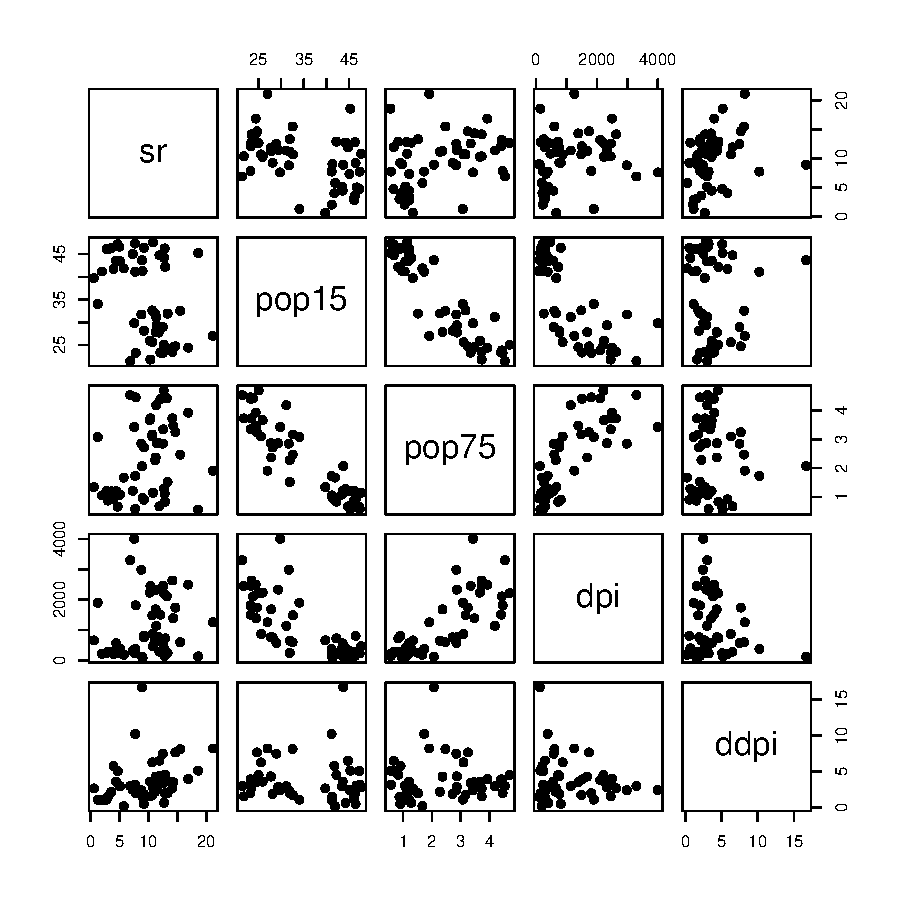
\includegraphics[width = 0.6\textwidth]{images/cancor}
\caption{Pairwise scatterplots of Life Cycle Savings data}
\end{center}
\end{figure}

And it is worth examining the correlation matrix:

\singlespacing
\begin{verbatim}
> cor(LifeCycleSavings)
              sr       pop15       pop75        dpi        ddpi
sr     1.0000000 -0.45553809  0.31652112  0.2203589  0.30478716
pop15 -0.4555381  1.00000000 -0.90847871 -0.7561881 -0.04782569
pop75  0.3165211 -0.90847871  1.00000000  0.7869995  0.02532138
dpi    0.2203589 -0.75618810  0.78699951  1.0000000 -0.12948552
ddpi   0.3047872 -0.04782569  0.02532138 -0.1294855  1.00000000
\end{verbatim}
\onehalfspacing

It appears that the \textbf{X} variables are correlated.   This is less so for \textbf{Y} variables, and even less so for \textbf{X,Y} inter-correlations.

You need to be sure that the variables are \emph{scaled} before carrying out a canonical correlation analysis.   

\singlespacing
\begin{verbatim}
LifeCycleSavingsS <- scale(LifeCycleSavings)
pop <- LifeCycleSavingsS[, 2:3] ## The X matrix
oec <- LifeCycleSavingsS[, -(2:3)] ## the Y matrix
\end{verbatim}
\onehalfspacing

Having created an \textbf{X} matrix and a \textbf{Y} matrix, we now want to find linear combinations of \textbf{X} which have maximum correlation with \textbf{Y}.

\singlespacing
\begin{verbatim}
> cancor(pop, oec)
$cor
[1] 0.8247966 0.3652762

$xcoef
             [,1]       [,2]
pop15 -0.08338007 -0.3314944
pop75  0.06279282 -0.3360027

$ycoef
           [,1]        [,2]         [,3]
sr   0.03795363  0.14955310 -0.023106040
dpi  0.12954600 -0.07518943  0.004502216
ddpi 0.01196908 -0.03520728  0.148898175

$xcenter
        pop15         pop75 
-4.662937e-16  2.753353e-16 

$ycenter
          sr          dpi         ddpi 
1.421085e-16 6.661338e-17 4.440892e-16 
\end{verbatim}
\onehalfspacing

This indicates one canonical correlate with a correlation of 0.8247966 between $z_{\boldsymbol{X}1}$ and $z_{\boldsymbol{Y}1}$

\begin{eqnarray}
z_{\boldsymbol{X}1} =  -0.08338007  x_{pop15} + 0.06279282 x_{pop75}\\
z_{\boldsymbol{Y}1} = 0.03795363 y_{sr} + 0.12954600 y_{dpi} +  0.01196908 y_{ddpi}
\end{eqnarray}

If we extract the coefficients as vectors (this time we have created \texttt{LCS.cancor} as an object; also we have used \texttt{as.numeric(\ldots)} to extract the coefficients in a form suitable for matrix multiplication).

\singlespacing
\begin{verbatim}
> LCS.cancor <- cancor(pop, oec)
> ycoef <- as.numeric(LCS.cancor$ycoef[,1])
> xcoef <- as.numeric(LCS.cancor$xcoef[,1])
> v1 <-  oec %*% ycoef ## remember oec and pop are scaled
> u1 <-  pop %*% xcoef
> plot(v1, u1)
> identify(v1, u1, row.names(LifeCycleSavings))
\end{verbatim}
\onehalfspacing


\subsection{Interpreting the canonical variables}

There is some ``controversy'' about the best way of interpreting the canonical variables.   You have two possibilities:

\begin{itemize}
\item Interpret the coefficients in a similar way to that used in principal components (problems with collinear variables)
\item Calculate the correlation between the canonical and the original variables (doesn't tell you anything about joint contributions)
\end{itemize}

%Consider:

%$\rho_{\hat{U},\boldsymbol{x}}$ = matrix of correlations between $\hat{U}$ and $\boldsymbol{x}$\\ 
%$\rho_{\hat{V},\boldsymbol{y}}$ = matrix of correlations between $\hat{V}$ and $\boldsymbol{y}$ \\
%$\rho_{\hat{U},\boldsymbol{y}}$ = matrix of correlations between $\hat{U}$ and $\boldsymbol{y}$ \\
%$\rho_{\hat{V},\boldsymbol{x}}$ = matrix of correlations between $\hat{V}$ and $\boldsymbol{x}$\\ 

%Which can be obtained fairly simply as:

%\begin{eqnarray*}
%\rho_{\hat{U},\boldsymbol{x}} = a \Sigma_{11}



\subsection{Hypothesis testing}

As with Principal Components, a certain amount of hypothesis testing is possible.   The distributional properties of canonical variables is far wilder than principal components - none of the recommended books discuss it.   However, the tests can be described.   For example, if we wanted to test whether there was any relationship between our two sets of variables:

\begin{displaymath}
H_{0}; \boldsymbol{\Sigma}_{12} = \boldsymbol{0}
\end{displaymath}

The Likelihood ratio test leads us to:

\begin{displaymath}
\Lambda^{\frac{2}{n}} = |\boldsymbol{I} - \boldsymbol{S_{22}^{-1}}\boldsymbol{S_{21}}\boldsymbol{S_{11}^{-1}}\boldsymbol{S_{12}}| = \prod_{i=1}^{k}(1-r_{i}^{2}) \sim \Lambda_{Wilks}(p, n-1-q,q)
\end{displaymath}

Using Bartlett's approximation this can yield a $chi^{2}$ test:

\begin{displaymath}
-\left(n-\frac{1}{2}(p+q+3)\right) \log \prod_{i=1}^{k}(1-r_{i}^{2}) \sim \chi^{2}_{pq}
\end{displaymath}


As we've seen before, perhaps we are more interested in finding out how many canonical correlations we need to keep in our analysis.   Bartlett also proposed a statistic only $s$ canonical correlations are non-zero:

\begin{displaymath}
-\left(n-\frac{1}{2}(p+q+3)\right) \log \prod_{i=s+1}^{k}(1-r_{i}^{2}) \sim \chi^{2}_{(p-s)(q-s)}
\end{displaymath}

%%% Local Variables: ***
%%% mode:latex ***
%%% TeX-master: "book.tex"  ***
%%% End: ***